\documentclass[
  bibliography=totoc,     % Literatur im Inhaltsverzeichnis
  captions=tableheading,  % Tabellenüberschriften
  titlepage=firstiscover, % Titelseite ist Deckblatt
]{scrartcl}

%irgendetwas mit Tabelen und Figuren anders Nummerieren 
\usepackage{chngcntr}
\usepackage{longtable} 

\usepackage{titling}

%Textdatein einfügen
\usepackage{verbatim}

% Paket float verbessern
\usepackage{scrhack}

% Warnung, falls nochmal kompiliert werden muss
\usepackage[aux]{rerunfilecheck}

% unverzichtbare Mathe-Befehle
\usepackage{amsmath}
% viele Mathe-Symbole
\usepackage{amssymb}
% Erweiterungen für amsmath
\usepackage{mathtools}

% Fonteinstellungen
\usepackage{fontspec}
% Latin Modern Fonts werden automatisch geladen
% Alternativ zum Beispiel:
%\setromanfont{Libertinus Serif}
%\setsansfont{Libertinus Sans}
%\setmonofont{Libertinus Mono}

% Wenn man andere Schriftarten gesetzt hat,
% sollte man das Seiten-Layout neu berechnen lassen
\recalctypearea{}

% deutsche Spracheinstellungen
\usepackage[ngerman]{babel}


\usepackage[
  math-style=ISO,    % ┐
  bold-style=ISO,    % │
  sans-style=italic, % │ ISO-Standard folgen
  nabla=upright,     % │
  partial=upright,   % ┘
  warnings-off={           % ┐
    mathtools-colon,       % │ unnötige Warnungen ausschalten
    mathtools-overbracket, % │
  },                       % ┘
]{unicode-math}

% traditionelle Fonts für Mathematik
\setmathfont{Latin Modern Math}
% Alternativ zum Beispiel:
%\setmathfont{Libertinus Math}

\setmathfont{XITS Math}[range={scr, bfscr}]
\setmathfont{XITS Math}[range={cal, bfcal}, StylisticSet=1]

% Zahlen und Einheiten
\usepackage[
  locale=DE,                   % deutsche Einstellungen
  separate-uncertainty=true,   % immer Unsicherheit mit \pm
  per-mode=symbol-or-fraction, % / in inline math, fraction in display math
]{siunitx}

\DeclareSIUnit{\channel}{Channel}
\DeclareSIUnit{\year}{a}

% chemische Formeln
\usepackage[
  version=4,
  math-greek=default, % ┐ mit unicode-math zusammenarbeiten
  text-greek=default, % ┘
]{mhchem}

% richtige Anführungszeichen
\usepackage[autostyle]{csquotes}

% schöne Brüche im Text
\usepackage{xfrac}

% Standardplatzierung für Floats einstellen
\usepackage{float}
\floatplacement{figure}{htbp}
\floatplacement{table}{htbp}

% Floats innerhalb einer Section halten
\usepackage[
  section, % Floats innerhalb der Section halten
  below,   % unterhalb der Section aber auf der selben Seite ist ok
]{placeins}

% Seite drehen für breite Tabellen: landscape Umgebung
\usepackage{pdflscape}

% Captions schöner machen.
\usepackage[
  labelfont=bf,        % Tabelle x: Abbildung y: ist jetzt fett
  font=small,          % Schrift etwas kleiner als Dokument
  width=0.9\textwidth, % maximale Breite einer Caption schmaler
]{caption}
% subfigure, subtable, subref
\usepackage{subcaption}

% Grafiken können eingebunden werden
\usepackage{graphicx}
\usepackage{wrapfig}

% schöne Tabellen
\usepackage{booktabs}
\usepackage[table]{xcolor}

% Verbesserungen am Schriftbild
\usepackage{microtype}

% Literaturverzeichnis
\usepackage[
  backend=biber,
  sorting=none
]{biblatex}
% Quellendatenbank
\addbibresource{lit.bib}
\addbibresource{programme.bib}

% Hyperlinks im Dokument
\usepackage[
  german,
  unicode,        % Unicode in PDF-Attributen erlauben
  pdfusetitle,    % Titel, Autoren und Datum als PDF-Attribute
  pdfcreator={},  % ┐ PDF-Attribute säubern
  pdfproducer={}, % ┘
]{hyperref}
% erweiterte Bookmarks im PDF
\usepackage{bookmark}

% Trennung von Wörtern mit Strichen
\usepackage[shortcuts]{extdash}

%\setcounter{tocdepth}{3} % + subsubsections



\author{%
  Benedikt Lütke Lanfer \\%
  \href{mailto:benedikt.luetkelanfer@tu-dortmund.de}{benedikt.luetkelanfer@tu-dortmund.de}%
  \and%
  Enno Wellmann \\%
  \href{mailto:enno.wellmann@tu-dortmund.de}{enno.wellmann@tu-dortmund.de}%
}
\publishers{TU Dortmund – Fakultät Physik}


\newcommand*\diff{\mathop{}\!\mathrm{d}}

\NewDocumentCommand \OverfullCenter {+m} {
\noindent\makebox[\linewidth]{#1} }

\usepackage{adjustbox}


% %Tabellen und Figuren Einstellung
% \counterwithout{table}{section}
% \counterwithout{figure}{section}
% \renewcommand{\thetable}{\Roman{table}}
% \renewcommand{\thefigure}{\Roman{figure}}

%Richtiges Einrücken
\setlength{\parindent}{0pt}


\title{V01:\\ Kosmische Myonen}
\author{Benedikt Lütke Lanfer \and Enno Wellmann}
\date{01.Juli 2024}
\publishers{TU Dortmund – Fakultät Physik}

\begin{document}
\begin{titlingpage}
    \begin{center}
        \begin{Huge}
            \textbf{\thetitle\\}
        \end{Huge}
    \end{center}
    \vspace{4cm}
    
\includegraphics[width=\textwidth]{Bilder/Logo_TU.png} \\
    \vspace{4cm}
    \begin{center}
        \begin{huge}
            \theauthor\\
        \end{huge}
        \vspace{0.5cm}
        \begin{Large}
            benedikt.luetkelanfer@tu-dortmund.de\\
            enno.wellmann@tu-dortmund.de\\
            \vspace{1.4cm}
            Bearbeitet: \today\\
            Durchgeführt: \thedate\\
            TU Dortmund – Fakultät Physik\\
        \end{Large}
    \end{center}
\end{titlingpage}
\tableofcontents
\newpage

\section{Zielsetzung}
In diesem Versuch wird ein Germanium Energiedetektor mit einer geeichten 152Eu
Quelle kalibriert. Der kalibrierte Detektor wird anschließend verwendet um das
Spektrum einer monochromatischen 137Cs Quelle aufzunehmen. Danach wird mit dem
Spektrum einer 133Ba Quelle deren Aktivität bestimmt. Schließlich wird anhand
eines weiteren Spektrums eine unbekannte Quelle identifiziert.

% Stichworte:
% \begin{itemize}
% \item Vollenergienachweiswahrscheinlichkeit
% \item Linien des Eu Spektrums
% \item Halbwertsbreite
% \item Compton Kante \item
% \end{itemize}

%---------------------------------------------------------------------------------------------------------------------------------------------------------------%

\section{Theorie}
\subsection[]{Wechselwirkung von Strahlung mit Materie}
Die Interaktionswahrscheinlichkeit von Gamma Strahlen mit Materie lässt sich
durch den Dämpfungskoeffizienten $\mu$ darstellen. Die Strahlungsintensität
fällt in dichten Materialien exponentiell ab $I ~ \exp(-\mu x)$. Dieser
Intensitätsverlust hängt direkt mit der Wirkungsquerschnitt des materials
zusammen und ist in $\mu$ eine additive Größe. Die Dämpfungskoeffizienten von
Gammastrahlen sind in Abbildung \ref{fig:mu} zu sehen.

\begin{figure}
	\centering
	\begin{subfigure}{.5\textwidth}
		\centering
		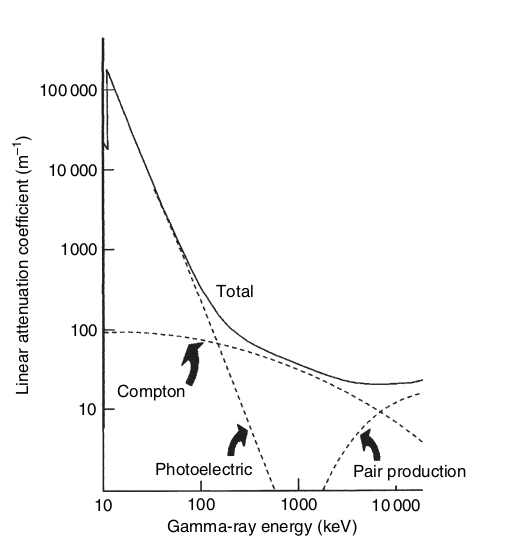
\includegraphics[width=0.9\linewidth]{./Bilder/E_mu_Gilmore.png}%
		\caption{Linearer Dämpfungskoeffizient aus \cite{book:gil}.}\label{fig:mu}
	\end{subfigure}%
	\begin{subfigure}{.5\textwidth}
		\centering
		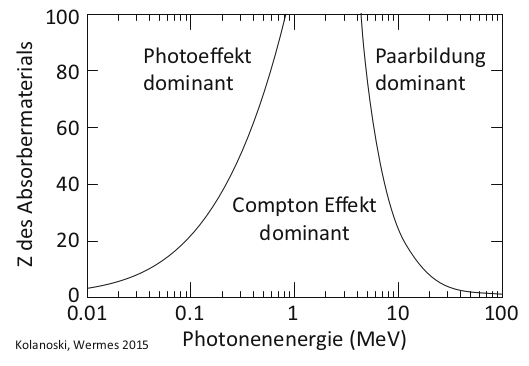
\includegraphics[width=0.9\linewidth]{./Bilder/E_Z_Kolanoski.png}
		\caption{Dominante Effekte nach $E_\gamma$ und $Z$ aus \cite{book:kolano}.}\label{fig:z}
	\end{subfigure}
	\caption{Interaktionswahrscheinlichkeiten von Gammastrahlen in verschiedenen Darstellungen.}\label{fig:zmu}
\end{figure}

Aus \cite{book:gil}. Die dominierenden Wechselwirkungen von Photonen mit
Materie sind die photoelektrische Absorption, die Compton Streuung und die
Elektronenpaarbildung. Bei der \textbf{photoelektrischen Absorption}
wechselwirkt das Photon mit einem im Atom gebundenen Elektron und befördert es
aus seinem gebundenen Zustand. Die Energie des Photons wird danach von dem
Elektron getragen und das Atom emittiert Strahlung, wenn es sich wieder abregt. Diese Interaktion
findet vor allem bei niederenergetischen Photonen statt. Eine grobe Annäherung
für das Verhalten der Wechselwirkungswahrscheinlichkeit ist der Term
\begin{align}
	\tau = \text{constant} \cdot \frac{Z^n}{E_{\gamma}^{m}}
\end{align} %TODO \tau mit dem linearen <Dämpfungskoeffizienten in Verbindung bringen.
wobei $m$ und $n$ zwischen 3 und 5 liegen \cite[vgl.][Kap 2.2.1]{book:gil}.
$\tau$ lässt sich hier in Verbindung mit dem linearen Dämpfungskoeffizienten bringen
\begin{align}
	\mu_{\text{PE}} = \tau \cdot \rho \cdot N_A /A
\end{align}

Die \textbf{Compton Streuung} ist in diesem Versuch aufgrund kleiner Energien
und großen $Z$ die häufigste Interaktion der Strahlung mit dem Material. Sie
ist (abhängig von $Z$) dominant bei Energien im Bereich von etwa
$\qtyrange{0.5}{10}{\MeV}$ Ihr differentieller Wirkungsquerschnitt wird durch die
Klein-Nishina-Formel beschrieben
\begin{align}
	\frac{d\sigma}{d \Omega} = Z r_0^2 \left(\frac{1}{1+\alpha(1-\cos\theta)}\right)^2
	\left(\frac{1+ \cos^2\theta}{2}\right)%
	\left(1+ \frac{\alpha^2(1-\cos \theta)^2}{(1+\cos^2 \theta)[1+\alpha(1-\cos(\theta))]}\right)
	\label{eq:wq_compton}
\end{align}% 
wobei $\alpha = h \nu / m_0 c²$ und $r_0$ der klassische Elektronenradius ist (vgl. \cite{book:knoll}).
Der Energieübertrag auf das Elektron wird berechnet durch
\begin{align}
	E_{e} = E_{\gamma} \left\{1- \frac{1}{1+ E_{\gamma}(1-\cos\theta)/m_0 c^2} \right\}
	\label{eq:ecompton}
\end{align}
Für diesen Versuch ist es wichtig, den Wirkungsquerschnitt der Comptonstreuung in Abhängigkeit der
Energie des gestreuten Elektrons $T = E_{\gamma} - E'_{\gamma}$ zu betrachten.
Hierfür wird in \cite[][Kap. 3.5.3]{book:kolano} die Klein-Nishina-Formel integriert.
\begin{align}
	\frac{d \sigma}{d T} =  \frac{\pi r_{e}^{2}}{m_e c^2 \epsilon}%
	\left[2 + \frac{t^2}{\epsilon^2(1-t)^2} + \frac{t}{1-t} %
		\left(t - \frac{2}{\epsilon} \right) \right]
	\label{eq:compton_energie}
\end{align}
Hier gelten $\epsilon = E_{\gamma} / (m_e c^2)$ und $t = T/ E_\gamma$.
Bei Rückstreuung des $\gamma$ Photons wird die Energie des Elektrons maximal
$T \rightarrow T_{max}$
Es ergibt sich im Spektrum die sogenannte Compton Kante bei

\begin{align}
	T_{CK}= E_\gamma \frac{2\epsilon}{1+2\epsilon}
	\label{eq:CK}
\end{align}

und der Rückstrahlpeak bei

\begin{align}
	T_{RP}= E_\gamma \frac{1}{1+2\epsilon}
	\label{eq:RP}
\end{align}

Bei Energien oberhalb der doppelten Ruhemasse des Elektrons ($\qty{1.02}{\MeV}$)
ist die \textbf{Elektronenpaarbildung} möglich. Diese Wechselwirkung tritt aber
nur bei sehr hochenergetischen Gammastrahlen auf (vgl \ref{fig:zmu}). Ihr
Wirkungsquerschnitt ist weit oberhalb der Eigenenergie konstant in $E_\gamma$
und proportional zu $Z^2$ des Absorbiermaterials \cite[vgl.][Kap
	3.5.5]{book:kolano}.

\subsection{Messung von Energie in Germanium Halbleiterdetektoren \cite{book:gil}}

Halbleiter Können durch das Bandstruktur Modell aus der Festkörperphysik
beschreiben werden. Elektronen befinden sich in einem Festkörper nicht auf
eindeutig festgelegten Energieniveaus, sondern auf Materialabhängigen
Energiebändern. Elektronen können die Energien zwischen diesen Bändern nicht
annehmen. Damit ein Strom in einem Material fließen kann, muss ein Elektron das
sogenannte Valenzband verlassen und ins Leitungsband des Materials wechseln. In
einem Halbleiter sind das Valenzband (das oberste voll besetzte Band) und das
Leitungsband durch eine Bandlücke in der Größenordnung von $\qty{1}{\eV}$
voneinander getrennt.
\begin{figure}
	\centering
	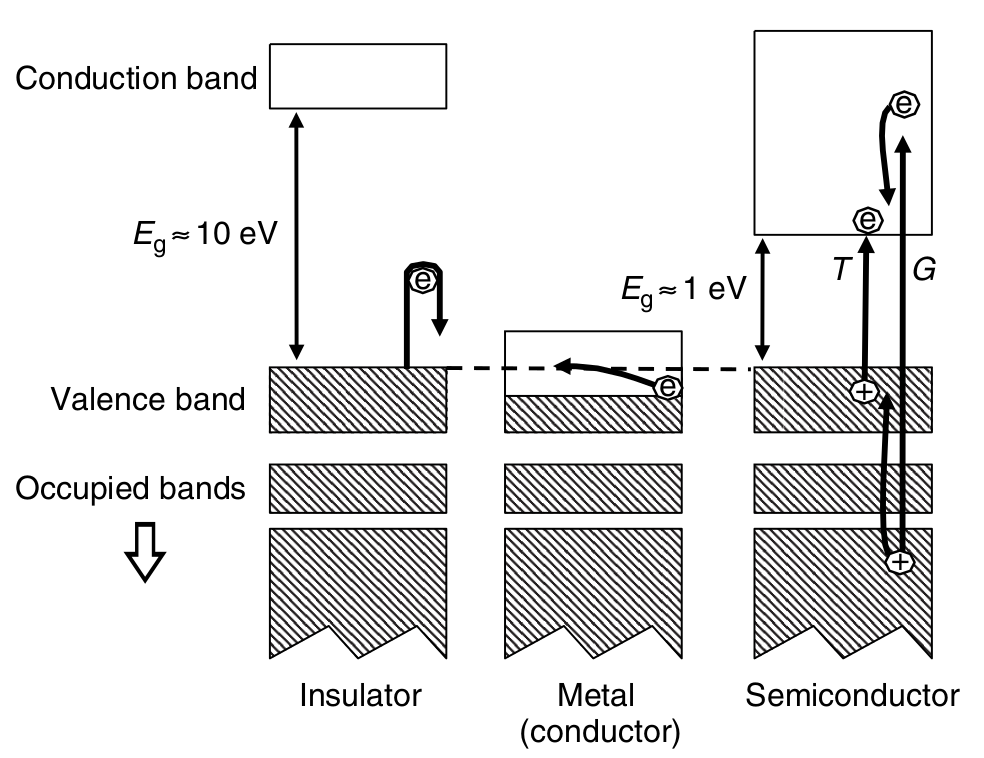
\includegraphics[width=0.4\textwidth]{./Bilder/ElectronBandsGilmore.png}
	\caption{Elektronen Bandstruktur aus \cite{book:gil}}\label{fig:eband}
\end{figure}
Das Leitungsband eines Halbleiters enthält meist auch Elektronen abhängig von
der Temperatur des Materials.
% Gleichung einfügen?
Um einen Halbleiter zu erhalten, der nach Möglichkeit nur von außen angeregte
Elektronen in seinem Leitungsband hat, ist es sinnvoll diesen so weit wie
möglich herunter zu kühlen. Gamma Strahlen erzeugen in der Interaktion mit dem
Detektor schnelle Elektronen, die durch das anregen von Bandelektronen ihre
Energie abgeben. Dieses Elektronen können in einem Germanium Halbleiter
Elektronenlochpaare erzeugen, wenn diese die notwendige Energie von $\epsilon =
	\qty{2.96}{\eV}$ erreichen. Die Anzahl an Elektronenlochpaaren ist mit
\begin{align}
	N = E_e / \epsilon
\end{align}

proportional zu der Energie $E_e$ des Elektrons. Basierend auf der Stärke des
Halbleiterstroms lassen sich so Rückschlüsse auf die Energie des Elektrons
ziehen.

\subsection{Form des Detektors \cite[vgl][Kap. 2.4]{book:gil}}

Die Größe des Detektors spielt eine wichtige Rolle darin wie die Energie des
$\gamma$ Photons in ein Spektrum von Elektronenenergien übersetzt wird. Für die
moderat Energiereichen $\gamma$ Strahlen werden für diese Diskussion nur der
Compton Effekt und die photoelektrische Absorption beachtet. In einem
idealisierten kleinen Detektor streuen die $\gamma$ Photonen nur einmal und
geben dabei entweder ihre gesamte Energie an ein Photoelektron oder einen Teil
der Energie an ein Compton gestreutes Elektron. Compton gestreuten
Gammastrahlen hinterlassen nur einen teil ihrer Energie in dem Germanium
Detektor, und verlassen diesen direkt danach wieder. Das Ergebnis ist ein
Spektrum in der Form des Compton Wirkungsquerschnitts $d\sigma/dN$ aus
Gleichung \eqref{eq:compton_energie}. Bei einem realistischen Detektor können
die Compton gestreuten Photonen im Prinzip noch weitere male mit dem Detektor
interagieren und so eine Elektronenenergie zwischen dem Vollenergiepeak und dem
erwarteten wert im Compton Kontinuum erreichen.

\subsection{Dateninterpretation}

Die Quellen werden mit einem festen Abstand $d$ zum zylinderförmigen Detektor
mit Radius $r$ eingespannt. Sie strahlen gleichmäßig in alle Richtungen ab
können aber nur im Kegelförmigen Raumwinkel des Detektors gemessen werden. Ist
$2\theta$ der Öffnungswinkel des Kegels so ist \cite{wiki:raum}
\begin{align}
	\Omega = 4 \pi sin^2\left(\frac{\theta}{2}\right) \\
	\theta = \arctan \left(\frac{r}{d} \right)
\end{align}\label{eq:raumwinkel}

Die Anzahl $Z$ an Messungen in einem bestimmten Energiepeak hängt von dem
Raumwinkel $\Omega$, der Emissionswahrscheinlichkeit $W$, der Aktivität $A$ und
der Vollenergienachweiswahrscheinlichkeit $Q$ ab. Die
Vollenergienachweiswahrscheinlichkeit ist eine wichtige Kenngröße des
Detektors. Sie ist das Verhältnis von Photoelektrisch absorbierten
Gammastrahlen, die ihre Energie vollständig abgeben und z.B. Compton gestreuten
Elektronen, die die Energie nur teilweise abgeben.
\begin{align}
	Z = \frac{\Omega}{4\pi} A T W Q
	\label{eq:Q}
\end{align}

Die entstehenden Peaks sind Poisson verteilt. Für große N können die
Histogramme aber mit einer Gaußverteilung angenähert werden. Bei den Peaks
lässt sich die Zehntelwertsbreite und die Halbwertsbreite bestimmen. Wenn es
sich bei diesen um gaußverteilte Werte handelt haben sie eine Halbwertsbreite
von $2\sqrt{2\ln 2} \sigma$ und eine Zehntelwertsbreite von $2 \sqrt{2\ln10}\sigma$.

% \subsection{Wahrscheinlichste Photonenenergien}

% \begin{itemize}
% 	\item[\ce   {^{152}Eu}] - \qty{ 40.1186 } {\keV} \qty{37.7 (5)}{\%}
% 	\item[\ce   {^{152}Eu}] - \qty{121.7817 (3)} {\keV} \qty{28.41 (13)}{\%}
% 	\item[\ce   {^{152}Eu}] - \qty{344.2785 (12)} {\keV} \qty{26.59 (12)}{\%}
% 	\item[\ce   {^{137}Cs}] - \qty{661.6553 (30)} {\keV} \qty{85.01 (20)}{\%}
% 	\item[\ce   {^{133}Ba}] - \qty{30.9731}{\keV} \qty{62.4 (7)}{\%} x ray peak
% 	\item[\ce   {^{133}Ba}] - \qty{356.0129 (7)}{\keV} \qty{62.05 (19) 	}{\%} breiterer peak
% 	\item[\ce   {^{125}Sb}] - \qty{427.88}{\keV} \qty{29.6}{\%}
% \end{itemize}
% \cite{web:lara}

\newpage
\subsection{Fehlerrechnung}
Für die Fehlerrechnung werden alle \textbf{Mittelwerte} von $N$ Messungen
folgendermaßen berechnet:

\begin{equation}
	\overline{x} = \frac{1}{N} \cdot \sum_{i=1}^N x_i
	\label{eqn:Mittelwert}
\end{equation}

und alle \textbf{Standardabweichungen zum Mittelwert} mit:

\begin{equation}
	\increment\overline{x} = \sqrt{\frac{1}{N\cdot(N-1)}\cdot\sum_{i=1}^N (x_i-\overline{x})^2}
	\label{eqn:St_Mittelwert}
\end{equation}

Bei einigen Messungen bzw Messdaten ist der Fehler auch schon im Vorhinein
angegeben. Der Fehler für zusammenhängende Messwerte wird dann mit der
\textbf{Gaußschen Fehlerfortpflanzung} berechnet:

\begin{equation}
	\increment{f} = \sqrt{ \sum_{i = 1}^{N}  \biggl(\frac{\partial{f}}{\partial{x_i}}\biggr)^2\cdot(\increment{x_i})^2}
	\label{eqn:Gauss}
\end{equation}

Die Fehlerfortpflanzung wird mit Uncertainties in Python \cite{uncertainties}
ermittelt.

%---------------------------------------------------------------------------------------------------------------------------------------------------------------%

\section{Durchführung \cite[vgl.][]{man:v18}}

Der hier verwendete Detektor ist Zylinderförmig (l= \qty{39}{\mm}, Durchmesser
= \qty{45}{\mm}) und befindet sich in einer Aluminium Schutzhülle. Der Abstand
des Detektors zur Schutzhülle beträgt \qty{1.5}{\cm}. Die Schutzhülle sorgt
dafür, dass Gammastrahlen mit einer Energie niedriger als etwa
\qtyrange{40}{50}{\keV} nicht gemessen werden können. Für die
Vollenergienachweiswahrscheinlichkeit werden nur Energien größer
\qty{150}{\keV} betrachtet. Im Inneren des Detektors befindet sich eine
Koaxiale Bohrung deren innere Oberfläche mit Gold bedampft ist. Dieser Metall
Kontakt sorgt für die Ausprägung einer Verarmungszone in dem Detektor, die
diesen zu einem effektiven Halbleiter macht.

\begin{figure}
	\centering
	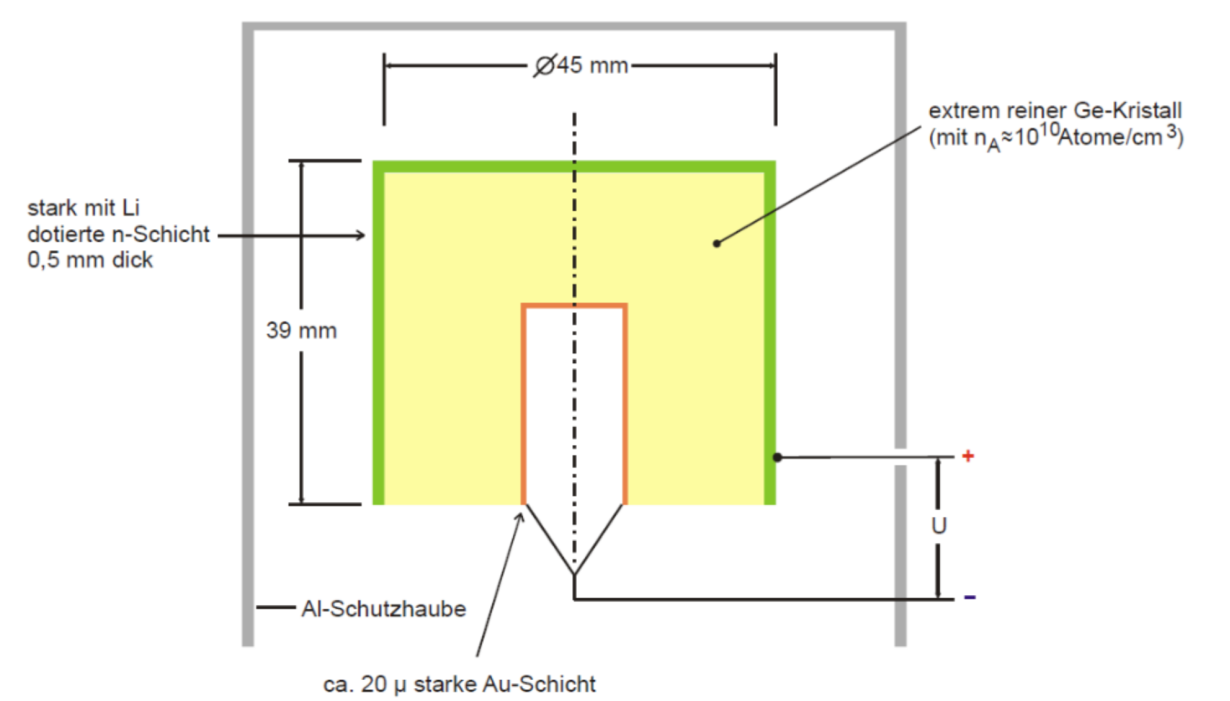
\includegraphics[width=0.4\textwidth]{./Bilder/querschnitt_detektor.png}
	\caption{Querschnitt des Germanium Detektors}\label{fig:cross}
\end{figure}

% TODO Abmessungen fertig machen

\subsection{Elektronik \cite[][Kap.17]{book:kolano}}
Der Detektor wird in diesem Versuchsaufbau durch vorgefertigte Bauteile
kontrolliert und ausgelesen. Ein Temperaturwächter kontrolliert die Kühlung des
Detektors und hält dessen Temperatur konstant auf $\qty{77}{\kelvin}$. Eine
Hochspannungsquelle erhält die Verarmungszone des Halbleiters aufrecht.
Um die Signale mit dem im PC eingebauten Viel-Kanal-Analysator detektieren können, 
müssen diese erst Analog verarbeitet und verstärkt werden. 
Dabei geht man hier wie folgt vor:

\begin{figure}
	\centering
	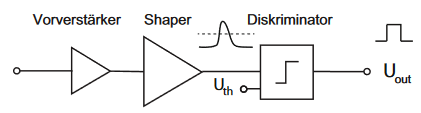
\includegraphics[width=0.8\textwidth]{./Bilder/Elektronik.png}
	\caption{Verarbeitungselektronik \cite{book:kolano}}\label{fig:elek}
\end{figure}

\begin{enumerate}
	\item \textbf{Vorverstärker:} Dieser verstärkt die Amplitude des gemessenen Signals, welches meist nur im Nanoampere Bereich ist. 
	\item \textbf{Der Shaper} verhindert die Überlagerung von Signal-Pulsen ($pile-up$) und verringert das Hintergrundrauschen. 
	Diese $pile-up$ können am Ausgang des Vorverstärkers entstehen, wenn ein weiteres Signal während seiner Abklingzeit eintritt.
	Durch eine Reihe von Hoch-/Tiefpässen können so die $pile-up$ in gaußförmige Pulse umgeformt ($shapen$) werden.
	Dieser Effekt wird im einfachsten Fall durch eine Reduzierung der Bandbreite der Signale erreicht.   
	\item \textbf{Diskriminator:} Um das Signal vom Rauschen zu filtern, wird ein Diskriminator eingesezt, welcher 
	die Signale oberhalb eines bestimmten Schwellwerts ($threshold$) durchlässt.
	Überschreitet das Signal diesen Schwellwert wird ein logisches Signal erzeugt. 
	Dies kann als Trigger für den Multichannel Analyzer verwendet werden.
	Auf diese Weise wird das weniger starke Hintergrundsignal herausgefiltert. 
\end{enumerate}

Diese Signale werden dann dem Computer übergeben, der mittels eines Viel-Kanal-Analysator ein Histogramm mit Zählrate in Abhängig vom Kanal erstellt.
Diese Kanäle müssen dann in der Auswertung, mittels des $\ce{^{152}Eu}$-Spektrums, nach der Energie Kalibriert werden.  

\subsection{Messprogramm}
Die Energiespektren von $\ce{^{152}Eu}$, der $\ce{^{137}Cs}$ und $\ce{^{133}Ba}$ werden
aufgenommen. Hierzu werden die Proben in einem Abstand von $\qty{70}{\mm}$ von
der Aluminium Abschirmung befestigt. Das Histogramm wird automatisiert jeweils
für etwa eine Stunde aufgenommen. Die genaue Messzeit wird in den Daten
automatisch hinterlegt. Schließlich wird die Unbekannte Quelle auf der
Schutzhülle positioniert. Deren Spektrum wird in gleicher Weise für etwa
$\qty{45}{\min}$ aufgenommen.
%---------------------------------------------------------------------------------------------------------------------------------------------------------------%

\section{Auswertung}
\subsection{Anmerkungen}
Die aufgenommenen Daten zur Myonenlebenszeit geben nicht den erwarteten Verlauf wieder und besitzen eine viel zu hohe Zählrate, als von Myonen zu erwarten.
Dieses liegt an einem Fehler beim Kalibrieren der Apparatur und dem Messen. 
Einer der Diskriminatoren die benutzt wurden, ist defekt und konnte nicht eingestellt werden. 
Dieses ist bei der Kalibrierung der Diskriminatoren uns nicht aufgefallen, sondern erst am Ende der Messzeit. 
Es wurde zwar versucht eine neue Messreihe, mit einem anderen kalibrierten Diskriminator, aufzunehmen, 
jedoch stürzte der PC mitten in der Messreihe ab, sodass die Daten verloren gingen. 
Eine dritte Messreihe hat nicht genug Datenpunkte um, eine Analyse zu beginnen. 
Daher wird mit dem fehlerhaften Datensatz gearbeitet und eine ungefähre Bestimmung der Lebensdauer von Myonen versucht.    

\subsection{Bestimmung der Verzögerungszeit}
Die aufgenommenen Zählraten \eqref{tab:data1} wurden gegen die jeweilige Verzögerungszeit $T_{vz}$ geplottet \eqref{fig:plt1} 
und das sich abzeichnende Plateau über den Mittelwert bestimmt. Dieser ergibt ein Wert von $\num{159.5}$ im Bereich von $\qty{4}{\us}$ bis $\qty{14}{\us}$.
Für die folgenden Messungen wurde eine Verzögerung von $\qty{10}{\us}$ gewählt, welches mittig im Intervall liegt. 

\begin{figure}[H]
	\centering
	\includegraphics[width=0.9\textwidth]{build/plot1.pdf}
	\caption{Verzögerungszeit Bestimmung}\label{fig:plt1}
\end{figure}

\begin{table}[H]
	\centering
	\begin{tabular}{c c}
		\toprule
		$T_{vz} \, [\unit{\us}]$ & $N $  \\
		\midrule
        0  & 128 \\
        1  & 123 \\
        2  & 118 \\
        4  & 157 \\ 
        6  & 151 \\
        8  & 149 \\
        10 & 169 \\
        12 & 156 \\
        14 & 179 \\
        16 & 118 \\
        20 & 85  \\ 
        24 & 44  \\
        32 & 29  \\
		\bottomrule
	\end{tabular}
    \caption{Messdaten der Versicherungsmessung}
    \label{tab:data1}
\end{table}

\subsection{Kalibrierung}

\begin{wrapfigure}{r}{0.6\textwidth}
	\centering
	\includegraphics[width=0.6\textwidth]{build/plot2.pdf}
	\caption{Kalibrierungsdaten}\label{fig:plt2}
\end{wrapfigure}

Die Kalibrierung des Viel-Kanal-Analysator ergab das in die nebenstehende Abbildung \eqref{fig:plt2} geplottete Spektrum. 
Der Doppelimpulsgenerator wurde immer um $\qty{0.5}{\us}$, beginnend bei $\qty{0.4}{\us}$ erhöht, daher hat jeder Peak im Spektrum diesen Abstand.
Die Peaks werden mittels  $find-peaks$ von $scipy$ \cite{scipy} bestimmt und danach die Zeit $t$ gegen die Channels aufgetragen. 
Dabei wird eine Ausgleichsgerade der Form $f(x)=m \cdot x+b$ durch die Messwerte gelegt und dessen Steigung bestimmt. 


\begin{figure}[H]
	\centering
	\includegraphics[width=\textwidth]{build/plot3.pdf}
	\caption{Ausgleichsgerade Kalibrierung}\label{fig:plt3}
\end{figure}


Die Parameter der Ausgleichsgerade

\begin{align*}
	m&=\qty{21,67(0,01)e-3}{\us\per\channel}\\
	b&=\qty{0,1651(0,0026)}{\us}
\end{align*}

werden im Folgenden benutzt, um die Channels in Zerfallszeit umzurechnen. 

\subsection{Lebensdauerbestimmung}
Wie bereits erwähnt sind die in Abbildung \eqref{fig:plt3} zusehenden Daten fehlerhaft. 
Neben einer viel zu hohen Zahlrate von Insgesamt $1.648.692$ innerhalb von einer Messzeit von $T_{mess}=\qty{157226}{\s}$,
weist das Spektrum eine ungewöhnliche Kante bei $t_k=\qty{1.075}{\us}$ auf.
Daher kann angenommen das die Myonensignale, gerade für kleine Zeiten $t<t_k$, von anderen unbekannten Signalen überlagert werden. 
Daher ist eine theoretische Berechnung des Hintergrundes unpraktisch, sondern dieser wird in den jeweiligen Ausgleichsrechnungen berücksichtigt. 
Im Folgenden werden verschiedene Methoden aus probiert, um die Lebensdauer zu extrapolieren. 
 
\begin{figure}[H]
	\centering
	\includegraphics[width=\textwidth]{build/plot4.pdf}
	\caption{Messdaten}\label{fig:plt4}
\end{figure}

Dazu ist das Spektrum in verschiedenen Bereiche unterteilt. 

\begin{enumerate}
	\item \textbf{Der rote Bereich} sind alle Daten die nicht benutzt werden, da sie entweder nach der Suchzeit $T_{such}=\qty{10}{\us}$ sind 
	oder sie zu random sind (Die Messwerte am Anfang), das eine Betrachtung keinen Nutzen bringt. 
	\item \textbf{Der blaue Bereich} ist deutlich höher als alle anderen Messwerte und weist einen steilen Abfall auf. ($\qty{0.533}{\us}<t_B<\qty{1.075}{\us}$)
	\item \textbf{Der cyane Bereich} wird durch ein Flachen linearen Abfall gekennzeichnet, 
	welcher am ehesten von der Messrate her auf Myonenzerfall hindeuten könnte. ($\qty{1.075}{\us}<t_B<\qty{10}{\us}$)
\end{enumerate}

\subsubsection{Der Cyan Bereich}
Der Bereich mit der ungewöhnlichen Kante wird ignoriert, da dessen Zählraten deutlich über die zu erwartenden Zahlraten von Myonen sind. 
Die Zählraten haben dabei jeweils den Fehler $\sqrt(N) $, welcher in allen kommenden Fits berücksichtigt wird. 
Der zu erwartenden Verlauf von dem Zerfall von Myonen ist ein exponentieller Abfall der Zahlrate oder in einem Logarithmischen Plot einen linearen Abfall. 
Dazu kommt ein möglicher Untergrund $U$ in den Messwerten, der zu berücksichtigt werden sollte. 
Deshalb wird eine exponentielle Ausgleichsrechnung der Funktion

\begin{equation}
	f(t)=N_0 \cdot \exp(-\lambda t) + U
	\label{eqn:exp}
\end{equation}

und eine lineare Ausgleichsgerade der Form

\begin{equation}
	g(t)=m \cdot t +b
	\label{eqn:lin}
\end{equation}

mittels $curfit$ von $scipy$ ermittelt. 
Der exponentiell Fit berücksichtigt dabei einen nicht trivialen Untergrund die lineare Ausgleichsgerade geht von einem vernachlässigbaren aus. 

\begin{figure}[H]
	\centering
	\includegraphics[width=\textwidth]{build/plot5.pdf}
	\caption{Bestimmung der Lebensdauer von Myonen im cyan Bereich}\label{fig:plt5}
\end{figure}

Die Parameter des exponentiellen Fit ergeben:

\begin{align}
	\lambda&=\qty{0.602(0.018)}{\per\us} &\Rightarrow & & \tau&=\frac{1}{\lambda }=\qty{1.66(0.05)}{\us} \\
	N_0&=\num{184(8)} \notag \\
	U&=\num{1.71(0.26)} \notag
\end{align}

und die der Ausgleichsgerade: 

\begin{align}
	m&=\qty{-0.438(0.014)}{\per\us} &\Rightarrow & & \tau&=\frac{1}{|m|}=\qty{2.28(0.07)}{\us} \\
	b&=\num{4.60(0.11)} &\Rightarrow & & N_0&=\num{100(11)} \notag
\end{align}

\subsubsection{Verbindung vom Blauen und den Cyanen Bereich}
Es soll nun versucht werden die ungewöhnliche Kante zu entfernen und danach eine weitere Ausgleichsrechnung durchzuführen. 
Dazu werden alle Messwerte im blauen Bereich um die ungefähre Höhe der Kante reduziert. 
Eine Betrachtung des blauen Bereichs allein ist nicht sinnvoll, da dieser definitiv keine Myonen widerspiegelt, sondern deren Signal nur überlagert. 
Die Überlegung hinter der Reduzierung des Gebietes ist diese Überlagerung zu verkleinern, ohne den charakteristischen Verlauf des Bereichs zu verändern. 
Es wird danach wieder die zwei Ausgleichsrechnungen \eqref{eqn:exp} und \eqref{eqn:lin} durchgeführt. 

\begin{figure}[H]
	\centering
	\includegraphics[width=\textwidth]{build/plot6.pdf}
	\caption{Bestimmung der Lebensdauer von Myonen im blau und cyan Bereich}\label{fig:plt6}
\end{figure}

\newpage
Diesmal sind die Parameter des exponentiellen Fit:

\begin{align}
	\lambda&=\qty{18.31(0.015)}{\per\us} &\Rightarrow & & \tau&=\frac{1}{\lambda }=\qty{0.0546(0.0005)}{\us} \\
	N_0&=\num{1.13(0.1)e10} \notag \\
	U&=\num{5.8(1)} \notag
\end{align}

und die der Ausgleichsgerade:

\begin{align}
	m&=\qty{-0.439(0.013)}{\per\us} &\Rightarrow & & \tau&=\frac{1}{|m|}=\qty{2.28(0.07)}{\us} \\
	b&=\num{4.61(0.11)} &\Rightarrow & & N_0&=\num{101(11)} \notag
\end{align}

%---------------------------------------------------------------------------------------------------------------------------------------------------------------%
\newpage
\section{Diskussion}


%---------------------------------------------------------------------------------------------------------------------------------------------------------------%
\newpage
\printbibliography

\end{document}